The game is built from the ground up to be played on the XBOX 360, but
has limited playability on Windows-based PCs.  An XBOX controller is
required to play this game.

We only distribute the source for this game, and as such the installation
procedure is somewhat complex, and has many prerequisites. We start off with
a quick description of the installation procedure, and give detailed steps in
later sections.

\subsection{Quick installation guide}

To play on PC:
\begin{itemize}
    \item Ensure both Visual Studio 2010 and XNA Game Studio 4.0 are installed
    \item Open the solution \emph{progark-spill} in VS.
    \item Build the solution (Key shortcut F6)
    \item Run without debugging (Key shortcut Ctrl+F5)
\end{itemize}

To play on XBOX 360:
\begin{itemize}
    \item Follow the first three steps for PC.
    \item Download and install \emph{XNA Creators Club} on your XBOX.
    \item Launch XNA-CC on your XBOX, and pair with development machine.
    \item When XNA-CC is awaiting a connection, choose \emph{Deploy} in
          VS.
    \item Finally, choose Run without debugging in VS.
    \item The game is now installed, and on following launches should
          be found in the XBOX' Game Library.
\end{itemize}

\subsection{Playing the game}

In the game, you should now see the main menu. It lists all connected 
controllers, and thus potential players. Each player that wishes to join the
game, must press the button \emph{A} on their controller. When you are ready,
press \emph{Start} on player ones' controller to launch the game.  You may quit 
the game from this menu by pressing the \emph{Back} button.  This
description has unfortunately not been added to the menu itself, due to
time-constraints.

% TODO:  Add ingame shot for context?
\begin{figure}
    \begin{center}
    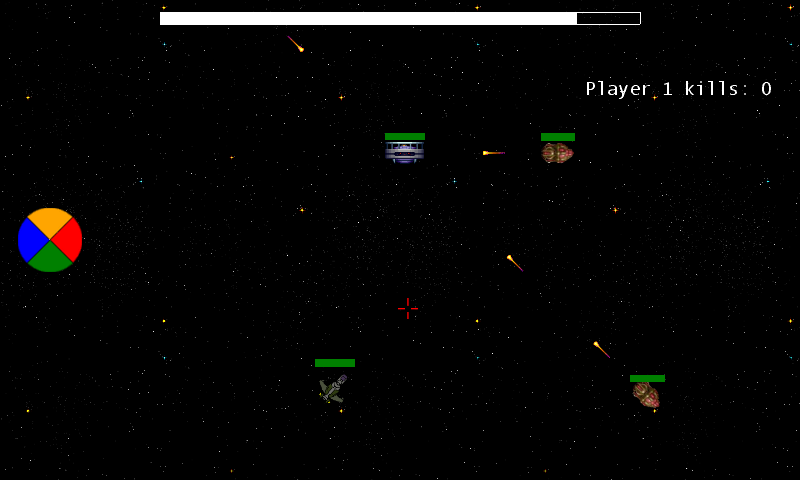
\includegraphics[width=\linewidth]{graphics/ingame}
    \caption{The main screen of the game}
    \label{fig:ingame}
    \end{center}
\end{figure}

You should now be playing the game. At any time you should be able to press
the \emph{Back} button to return to the main-menu, or \emph{Start} button to
pause the game. Pressing \emph{Back} when the game is paused returns you to
the game.

In the center of the screen you should see the objective, which you must 
defend. You should also see a spaceship for each player which joined the game.
You control your spaceship with the \emph{Left Stick} of your controller.
The spaceship always faces the crosshair, which you can move around using
your \emph{Right Stick}. You can shoot using your \emph{Right trigger}.

Along the top of your screen you should see a bar, representing the time
left of this level. When it reaches zero, and all enemies have been destroyed
you win the level (and in the case of the demo-level, the game itself).
Should the objective be destroyed, you lose the game.

On the left edge of the screen you can see which abilities you may use.
This UI element records the time until you can use an ability, by filling
pieces of a pie-chart. The pies are color-coded to buttons on your controller.
A white ring surrounding the pies means you have leveled up, and can improve
one of your abilities.You do this by pressing the corresponding direction
on you \emph{D-Pad}

There are two ways two play the game, either by deploying the game to the Xbox 360 and play it on the console, or 
run the game on Windows with two Xbox 360 controllers attached. We have written a manual for both, so the reader can 
test the game according to his/her preferences. 

\subsection{Xbox 360}

In order to play the game on the Xbox 360 Console, there are several prerequisites to take into account. Firstly, 
the following is mandatory\cite{deploy}:

\begin{itemize}
	\item Computer running Windows with XNA Game Studio 4.0 
	\item Xbox 360 Console with two controllers
	\item XNA Game Studio Connect on the Xbox 360 Console 
	%\item Atleast an Silver Xbox LIVE membership \\
	%\item XNA Creators Club premium membership \\
	\item Hard drive on the Xbox 360 to deploy the game onto 
\end{itemize}

\subsubsection{Connecting the Xbox 360 Console with XNA Game Studio 4.0}

Note! In order to download \textbf{XNA Game Studio Connect}, the Xbox 360 console needs an internet connection. \\

\begin{enumerate}
	\item On the Xbox 360 Console, navigate to \textbf{Game Marketplace}.
	\item Select \textbf{Explore Game Content} and then \textbf{Browse}. 
	\item When your at the \textbf{All Games} screen browse to \textbf{Genre} and select \textbf{Other}. 
	\item Scroll to \textbf{XNA Creators Club} and select it. 
	\item From this pane, select \textbf{All Downloads}, then select \textbf{XNA Game Studio Connect}. 
	\item \textbf{Confirm Download} to begin downloading. 
\end{enumerate}

In order to deploy the game to the Xbox 360 console, the development computer and the Xbox 360 needs to be on the same subnet on the local network. If the computer and console is behind the same router, it is very likely that you're on the same subnet. In order to deploy the game a \textbf{connection key} needs to be generated. \\

\begin{enumerate}
	\item On the Xbox 360 Console, go to \textbf{My Xbox} and select \textbf{Game Library}. 
	\item then go to \textbf{Collections} tab and select \textbf{Community Games}. 
	\item Select \textbf{XNA Game Studio Connect} and then select \textbf{Launch}. 
	\item The XNA Game Studio connect screen will appear: \\ \begin{center}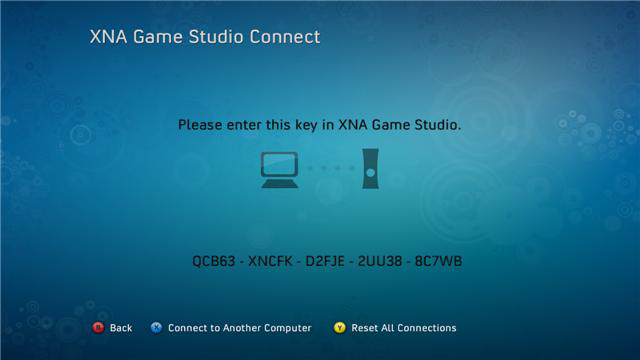
\includegraphics[scale=0.5]{graphics/connect}\end{center}
	\item If a \textbf{Connection Key} is displayed go to step \ref{generated}. 
	\item If the \textbf{Connection Key} does not appear, the Xbox 360 console could already be connected to this computer. The game studio supports multiple connection keys for multiple computers. To add a new connection press \textbf{X}. 
	\item \label{generated} On your computer, go to the \textbf{Start} menu, select \textbf{programs} and then select \textbf{XNA Game Studio 4.0}. 
	\item Launch the \textbf{XNA Game Studio Device Center}.
	\item Click \textbf{Add Device} \\ \begin{center}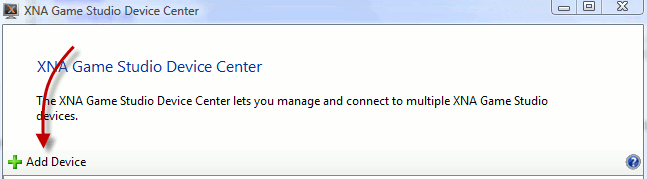
\includegraphics[scale=0.75]{graphics/add_device}\end{center} 
	\item Select the type type of device to be \textbf{Xbox 360} \\ \begin{center}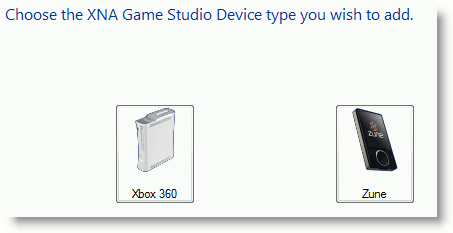
\includegraphics[scale=0.75]{graphics/type_of_device}\end{center} 
	\item Enter a name for the console and press \textbf{Next}. 
	\item Enter the connection key that is displayed in the XNA Game Studio Connect on the Xbox 360 console. 
	\item Once you have typed in the correct key, press \textbf{Next} on the \textbf{XNA Game Studio Devices} dialog box. 
	\item The XNA Game Studio Device center will test the connection. If it fails, pay attention to the error message of the dialog box. If it did not result from a mismatched key, please refer to \cite{troubleshoot}. 
	\item Click \textbf{Finish}. The console will now be listed in the XNA Game Studio Device Center  
\end{enumerate}

\subsubsection{Deploying the game to Xbox360}

\begin{enumerate}	
	\item On the development computer, fire up the project in Visual Studio.
	\item Then go to the Xbox 360 console and go to \textbf{My Xbox} and then select \textbf{Game Library}. 
	\item From \textbf{Game Library}, go to the \textbf{Collections} tab and then select \textbf{Community Games}
	\item Select \textbf{XNA Game Studio Connect} and then select Launch, which will display a screen like this: \\ \begin{center}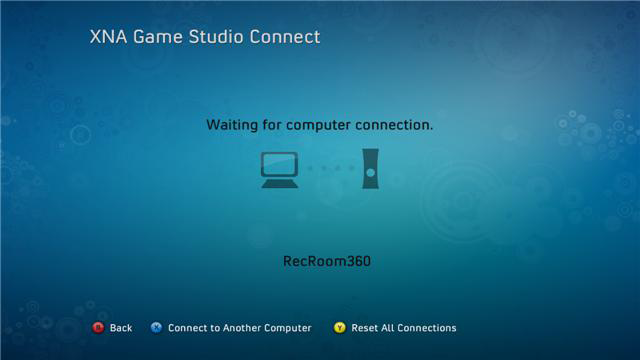
\includegraphics[scale=0.5]{graphics/connect2}\end{center}
	\item On your computer, build the project, deploy the needed files Xbox 360 and then run.
	\item Now you have deployed the game. 
	\item The game will appear in \textbf{Recent games} in the \textbf{Game Library}.	 
\end{enumerate}

\subsection{Playing the game on a (Windows) computer}

In order to play the game on a Windows computer, you need at least two Xbox 360 controllers. To connect a controller to the PC, you will need a USB cable connector from the controller to the computer. From this point, simply execute the executable file, and play! 
